In this chapter, we will discuss the issue of aggregation by focusing on
input-output statistics. The production network of an economy has been
a subject of intense recent study. One long standing issue concerns
the origin of macro-economic fluctuations: the traditional view of the
GDP as the sum of many weakly dependent random shocks clashes with the
observation that GDP fluctuations are markedly non-gaussian in the
tails \cite{non-gaussGDP}. Ref. \cite{Gabaix} invoked the extreme
heterogeneity of firm sizes, suggesting that shocks in a single large
firm can account for the observed distribution.  Acemoglu {\em et al.}
\cite{Acemoglu12} instead noticed that propagation of shocks across
the input-output production network can also reproduce non-gaussian
fluctuations in GDP.

We collected extensive data on the production network of a wide range
of countries for different years.  A central quantity in input-output
economics is the direct requirement matrix $D$ (see \cite{Acemoglu12,BEA_handbook}), a square matrix with order equal to the number of
goods $M$ available in the data. Each element $D_{\mu\nu}$ of the
direct requirement matrix is the amount of dollars (or euros) needed
of good $\mu$ to produce one dollar of good $\nu$ in the economy. The
matrix generates a weighted, directed graph of dependencies between
goods, which allows one to quantify the cascade effect of isolated
shocks in the economy, i.e., how much does a 50\% decrease in oil
prices affect the production capabilities of goods that directly use
oil as an input, and how this shock spreads to goods that are produced
using outputs of oil intensive industries.

The sum of the elements of the direct requirement matrix along a
column yields the {\em degree} of the good in the corresponding row,
which quantifies its level of dependence on other inputs.  The first
result we find is that, in a wide range of economies,
degrees follow an exponential distribution ({\em universality}). This
is suggestive, as this is the maximum entropy distribution consistent
with sole knowledge of that the average degree is fixed to one, by row
normalisation.  Furthermore we show that such a maximum entropy
distribution arises from aggregation, which is established both by
studying a dataset where the input-output network is known at a finer
resolution and by studying aggregation in a model of large random
economies.  The convergence to the exponential distribution depends on
how the aggregation is carried out and this has important consequences
on the estimate of aggregated fluctuations: classification methods
currently employed by the economic agencies may lead to underestimated
aggregate fluctuations.


\section{Input-Output Economics: Definitions and stylised facts}
\label{sec:IO}

The data we will focus our analysis on in this chapter are the Input-Output tables published by
the Bureau of Economic Analysis (BEA) for the United States and by the
Eurostat for the European Union. The Input-Output tables are part of a country's national accounts, and they flow of intermediate and final goods between different producing sectors in an economy. More specifically, in these tables, all the industries
and commodities of a country are aggregated into sectors, such as
``Agriculture, hunting and related services'', ``Financial services,
except insurance and pension funding'', etc. The tables then describe how much of each type of good these industries consume (i.e., use as an Input) for their operations, and how much they producte (i.e., have as Output). 

The classification system employed for categorizing the different sectors of the economy, the NACE\footnote{Acronym for \emph{Nomenclature statistique des activités économiques dans la Communauté européenne}} for the EU and the NAICS\footnote{\emph{North American Industry Classification System}} for North America, is the
same for both industries and goods, and are each defined in different levels of
aggregation: the 2007 US data, for example, is available at the
detailed, aggregated and summary levels, with 389, 71 and 15 different
sectors respectively. In the NAICS, the sector "Mining" in the summary level of aggregation (with the whole economy split into 15 sectors) breaks down to "Oil and gas extraction", "Mining, except oil and gas" and "Support activities for mining" at the aggregated level. Then, in the detailed level, is further broken down into 8 categories, some of which are "Coal mining", "Iron, gold, silver, and other metal ore mining", etc. The EU data has the same characteristics, except it is only available at the 64 and 10 sector aggregation levels.

The main raw data available online \cite{bea_data, eurostat_data} are two matrices named Make (or Supply) and Use tables,
which we will refer to as $M$ and $U$ respectively. $M_i^\mu$ is the
amount of euros (or dollars) that the industries of sector $i$ produce
of good $\mu$ and $U_i^\mu$ is the monetary amount of good $\mu$ that
industries in sector $i$ use for their production. In a simplified version of the
economy that would disregard, among other things, wages, capital
devaluation and taxes, the profits of a sector $i$ would be given
simply by $\sum_\mu (M_i^\mu - U_i^\mu)$.

For the European Union, we used the workbooks of
nine countries: Austria, Denmark, Finland, France, Germany, Greece,
Italy, Netherlands, Spain. Other countries considered were
Ireland, Portugal, Sweden and the United Kingdom, but the data for
these countries has a significant part omitted for
confidentiality reasons, so these countries were discarded. For every country there were two tables of output (the "Use" tables) available for each year:
one at the seller's prices and one at the purchaser's prices. The latter was used for all purposes.

We are particularly interested in the interdependence between the goods,
and for that purpose we follow the BEA handbook and construct a product-by-product Direct Requirements table
\cite{BEA_handbook}, which will give us how many dollars we need of
one good to produce one dollar of another. We first build the product-by-industry Direct Requirement matrix by
dividing each company's usage of goods by its total outputs, that is:

\begin{equation}
  \label{eq:dr_ic}
  B_i^\mu = \frac{U_i^\mu}{\sum_{\nu=1}^M M_i^\nu}
\end{equation}

The matrix $B_i^\mu$ gives us how many dollars of product $\mu$ we need to
produce one dollar of industry $i$'s output. We then define the
Market Share matrix, which is simply the fraction
of a given good that a company produces:

\begin{equation}
  \label{eq:market_share}
  W_i^\mu = \frac{M_i^\mu}{\sum_{j=1}^N M_j^\mu}
\end{equation}

Given these two matrices, we sum over the firms to define the product by product Direct
Requirement matrix, given by $D = B W$, that is:

\begin{equation}
  \label{eq:D}
  D_{\mu\nu} = \sum_{i=1}^N \frac{U_i^\mu}{\sum_{\eta=1}^M M_i^\eta} \frac{M_i^\nu}{\sum_{j=1}^N M_j^\nu}
\end{equation}

Each element $D_{\mu\nu}$ of the direct requirement matrix is a sum of
the firms direct requirements of $\mu$ weighted by their market share
on $\nu$. This gives us how many dollars of good $\mu$ are used in the
economy for the production of one dollar of good $\nu$.

This matrix therefore defines a directed weighted
graph on the goods, with the incoming edges of $\mu$ being its inputs
and the outgoing edges its usage by other products in the
economy. Therefore it's natural to characterize goods by their
indegrees, the weighted sum of the incoming edges, and the outdegree,
the weighted sum of the outgoing edges. That is:

\begin{equation}
  \label{eq:io_1}
 d'_\nu = \sum_{\mu=1}^M D_{\mu\nu},  \quad  d_\mu = \sum_{\nu = 1}^M D_{\mu\nu}
\end{equation}

The indegree $d'_\nu$ is how many dollars are used to produce one
dollar of a certain good. This defines the profitability of the good,
minus salary and wages, so we expect that for every good $d'_\nu \leq
1$. In a perfect competitive market, one would have $d'_\nu = 1$.

The outdegree $d_\mu$ is a more interesting quantity. It gives us the
total amount of dollars of good $\mu$ used in the economy (given that
each good requires \$1 to be produced). In a sense, high outdegree
goods are ``structural'' and very necessary for production, while low
outdegree goods are less so. Note that this does not mean that they
are unimportant. Retail services, for example, have outdegree equal or
close to zero in all data analysed in this paper. This is because no firm
uses retail stores services as an input to its production, all of
the sector's output is used as consumption in the
economy, clearly it does not mean it's an irrelevant sector. It does
mean, however, that a sudden closure of half of the retail stores in
an economy would certainly have a much smaller effect than the
equivalent shock in other goods such as energy and financial
services. In loose terms, this suggests that high outdegree sectors
are more systemically important than low degree ones.

In \cite{Acemoglu12} Acemoglu \emph{et al} used the US direct requirement
tables produced in a model economy to quantify how susceptible the American
economy is to independent normally distributed random shocks. In that paper, they challenged the standard notion in Macroeconomics that these shocks are self averaging and cancel themselves out. Instead, what was shown is that, in the context of their production model,
independent shocks do not average out when the outdegree distribution
has heavy tails. Therefore aggregate fluctuations remain large even in
the limit of large economies. Before addressing these issues, we
 first discuss the degree distribution that emerges from
empirical data.

\subsection{Universality of the degree distribution}

In order to relate to their results, we follow \cite{Acemoglu12} and
normalize all the indegrees to unity so we are able to compare the
data with a Random Economy model's competitive equilibrium. We
therefore only look at the outdegrees, from now on, that we simply call
degrees \footnote{We found qualitatively similar results even
  without this normalization}.

We plot on figure \ref{fig:6countries} the counter cumulative distribution
of the degrees $P(d < x)$ in a semi-log scale for six out of fourteen
OECD countries for which we obtained the Input-Output data. Also plotted is the
respective linear regression, in which the slopes are a very good fit
close to the degree average $\overline{d}=1$, suggesting that most of the
distributions have an exponential shape. The two main outliers from
the exponential law in our data, the US and Germany, are shown in the
figure.

To better illustrate this universal feature of the distributions, we
derive two main quantities for each country (we refer the reader to
Appendix \ref{app:stat} for more details on the statistical measures used throughout the chapter): The first is the $p$-value in a Kolmogorov-Smirnov 
test against an exponential distribution.% if we assume that the country degrees are random exponential variables. 
When $p$ is very small the hypothesis that the degrees come from an
exponential distribution should be rejected. 

The second quantity we use is derived from the Bayesian Information Criterion (BIC)
\cite{Kass95}. This compares different models from which the data may have been generated,
by computing the difference $\Delta$BIC in the log-likelihoods corrected by the BIC term which accounts for
the different complexity of the models. 
Specifically, in Figure \ref{fig:BICpval}, we compare the exponential distribution with a Gaussian distribution. 
This choice derives from the fact that one may naively expect that, upon aggregation, degrees 
behave as sums of random variables and hence should ultimately converge to Gaussian variables. 


\begin{figure}[!ht]
  \centering
  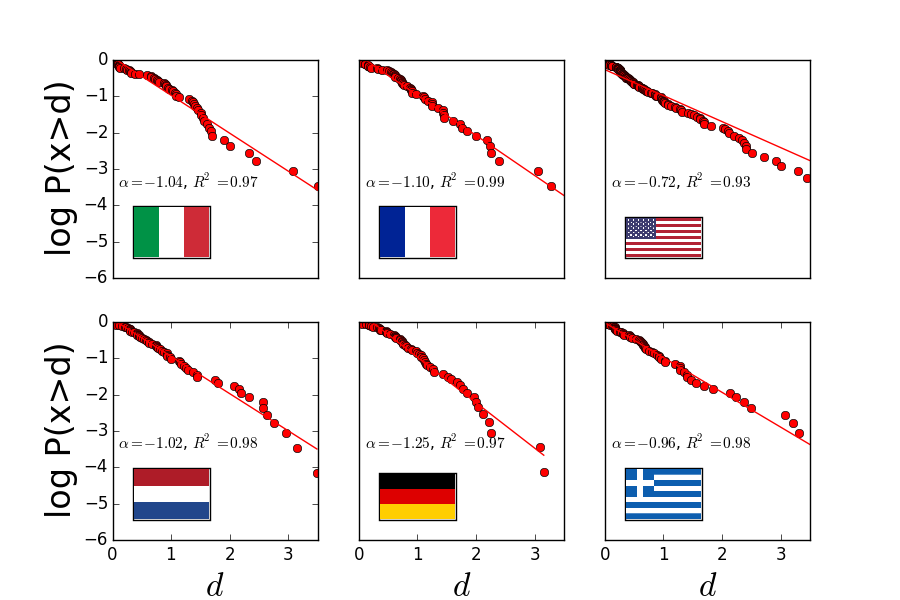
\includegraphics[width=0.95\textwidth]{figs_io/6panel_data.png}
  \caption{Outdegree distribution of several countries. The data shown
    is the counter cumulative in semilog scale, along with the linear
    fit. The largest outliers of our data, the US and Germany, are
    shown here.}
  \label{fig:6countries}
\end{figure}

\begin{figure}[!ht]
  \centering
  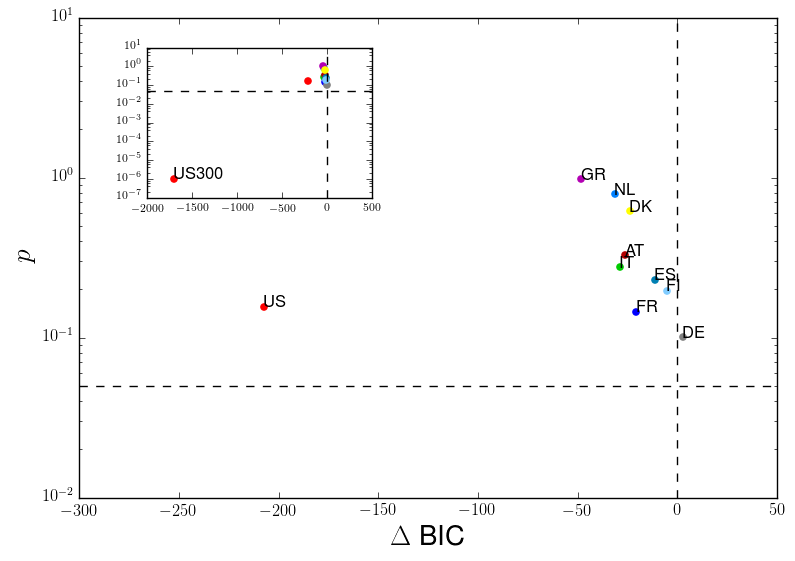
\includegraphics[width=0.95\textwidth]{figs_io/bic_pval_countries.png}
  \caption{Countries sorted by $\Delta$BIC of gaussian vs exponential
    (x axis) and probabilities of KS distance against exponential (y
    axis). Inset: same plot with the US $M=300$ level of
    disaggregation included. Dashed lines indicate $\Delta$BIC$=0$ and
    $p=0.05$.}
  \label{fig:BICpval}
\end{figure}

Figure \ref{fig:BICpval} depicts $p$ versus $\Delta$BIC for all the countries studied. We see that the bulk of the EU countries lie together in a
small cluster of the graph, indicating that the exponential hypothesis
is a very good fit for them. This is further confirmed
by putting the finer resolution data for the United States
(represented by the US300 point) in the same plane: the disaggregated
distribution is a very strong outlier compared to the coarser data.

A more careful analysis at the ``exponential bulk'' shows that the
main outliers are the US data, that exhibits a distribution bending
upwards in the semi-log plot of Figure \ref{fig:6countries}, and
Germany with a degree distribution bending downward. This motivated us
to carry out the BIC test between the exponential distribution
hypothesis and a stretched exponential defined as

\begin{equation}
\label{eq:stretched_exp}
P(d)=A(b,\theta)e^{-b x^\theta},\qquad b,\theta>0
\end{equation}

The result of this BIC test is shown in Figure
\ref{fig:theta_pval_data}, where the shaded region is where the
exponential ($\theta = 1$) is preferred to the stretched exponential
($\theta \neq 1$). We see that all countries analysed lie in this
region, with the exception of the US -- that is best fitted with $\theta<1$ -- and
Germany, Spain and Finland -- that are best fitted with $\theta>1$.

An exponential degree distribution across most of the countries under
study is of major relevance because the average degree of these
datasets is set to one by the normalisation requirement $d_\mu'=1$,
and the distribution of maximal entropy consistent with this
constraint is the exponential distribution. Since this is the least
informative distribution given the constraints we have, this suggests
that all the details of the input-output economics at the microscopic scale
have been washed out in the aggregation process.

Of course, the fact that this is the least informative doesn't mean
there is no information available. One can learn important things
about the economies in the aggregated dataset by looking at the relative 
importance of the different sectors. For example, among the
high degree products, ``Financial services'', ``Legal and accounting
services'' and ``Chemicals and chemical products'' are the highest
ranking ones, whereas, ``Imputed rents of
owner-occupied dwellings'' and ``Retail trade services'' have zero
degree in all countries. One can also look at the structural
differences between countries: in France, for example, products of
``Security and investigation services; office administration; office
support and other business support services'' are twice as used as in
Italy (degree of 3 vs 1.69), whereas in Italy,
``Electricity, gas, steam and air-conditioning'' are twice as depended
upon as in France (degree 4 vs 2). Yet the fact that the distribution of
degree takes a form consistent with maximum entropy, suggests that
the distribution carries no specific information on the economy. 
We shall now argue that this information is actually "lost in aggregation"
by looking at how the degree distribution evolves at different level of aggregation.


\section{Loss of information via aggregation}
\label{sec:aggreg} 

The above results show that aggregated data have a less informative
distribution of degrees. Indeed, for the most disaggregated data
available -- the 2007 US economy with $M=382$ -- we find that the
distribution of degrees is further away from the exponential
distribution with respect to the US data with $M=64$ sectors (see
point US300 in Fig. \ref{fig:theta_pval_data}).  At the other extreme,
if at a certain level of aggregation the distribution is exponential,
when we aggregate further, we expect the distribution to converge to a
Gaussian limit, because the degree at the coarser level is the sum of
the degrees at the finer one. This is appropriate if the degrees are
weakly dependent random variables, which in turn depends on how the
aggregation process is carried out, i.e. which sectors are put
together at the finer scale.  To answer the question of whether the
loss of information depends on the manner in which the aggregation is
carried out we will artificially aggregate the goods in the Use and Make tables
described in Section \ref{sec:IO} by collapsing pairs of goods into a
single one, ie, if we collapse $\mu_1$ and $\mu_2$ into $\mu$ the new
Use matrix would be $N$ by $M-1$ and would have $U_{i\mu} = U_{i\mu_1}
+ U_{i\mu_2}$. We would like to compare aggregation in two extreme
cases \emph{(i) random}: we choose $\mu_1, \mu_2$ randomly and
\emph{(ii) ranked}: we choose the two most correlated goods via
Spearman rank of the $M - U$ matrix, so that goods that highly
correlate in the usage as inputs - outputs by the industries will be
aggregated together first. In loose terms, as suggested by the
previous argument, we expect a faster loss of information
(i.e. convergence to the exponential distribution) when the
aggregation is carried out without taking into account the structure
of the data. As we'll discuss, this has practical consequences,
because a standardised aggregation method that has to be applied to
many countries, such as the one used in EU, may determine a faster
convergence to an uninformative distribution than a method that is
tailored to fewer countries (the one used by the US, Canada and
Mexico).

\begin{figure}[!ht]
  \centering
  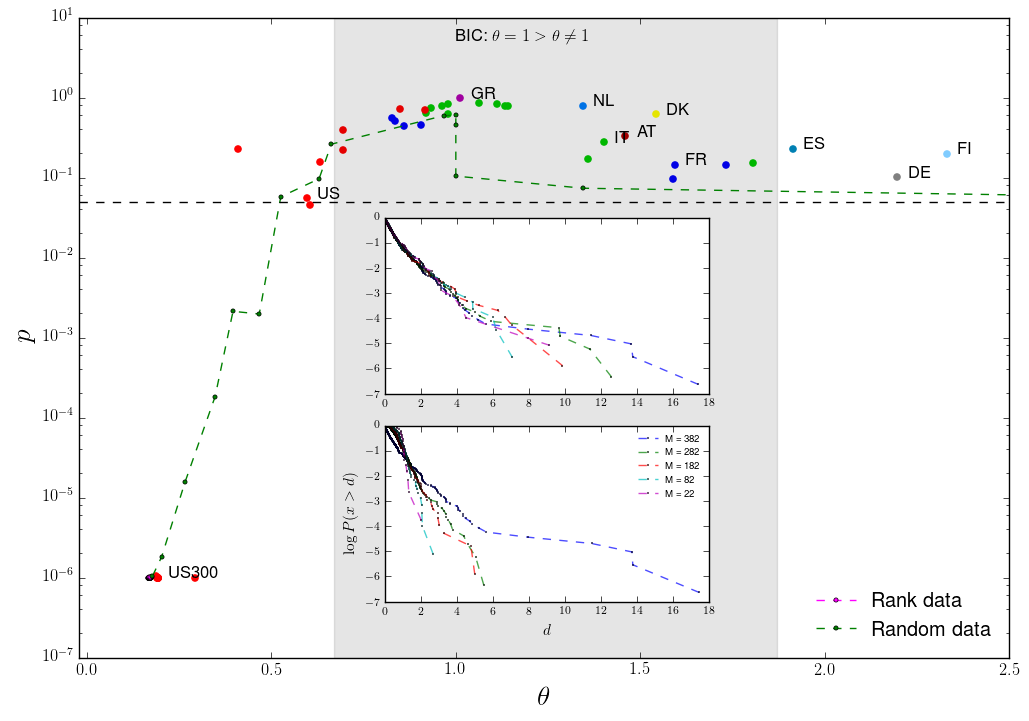
\includegraphics[width=0.95\textwidth]{figs_io/theta_pval_data_agg_w_inset.png}
  \caption{Countries in the $(p, \theta)$ plane, along with the two
    artificial aggregation processes carried out on the US300 data. The shaded
    area is the region where the BIC favors exponential distribution
    ($\theta = 1$) as opposed to stretched ($\theta \neq
    1$).
    \emph{Insets}: Evolution of the degree distribution under rank
    (top) and random (bottom) aggregation.}
  \label{fig:theta_pval_data}
\end{figure}


\subsection{Empirical data: the case of the US}

We take the most disaggregated data available, the 2007 US economy
with $M=382$ sectors, and aggregate according to the two methods
described above.  The results in the $(p, \theta)$ plane
are shown in figure \ref{fig:theta_pval_data}. We observe that we indeed obtain very different behavior depending on how the aggregation is carried out. Interestingly, the artificial method closer to the BEA classification system is random aggregation, while the ranked aggregation never converges to the exponential distribution. This is
because it creates a very dense ``supergood'' with positive entries in
all of its Make and Use tables that has a very high degree, while the
rest of the goods are left with sparse entries in the
tables. Nonetheless, ranked aggregation preserves the maximum degree
observed in the economy, as shown in the insets of figure
\ref{fig:theta_pval_data}.

\subsection{Random economies}

We now turn to the question of whether one can reproduce the maximum entropy degree distribution with a simple model and what is the effect of aggregation in those artificial economies. For that, we will build Input-Ouput matrices for economies in the Random Linear Economy model described in chapter \ref{cha:RLE}.

\begin{figure}[!ht]
  \centering
  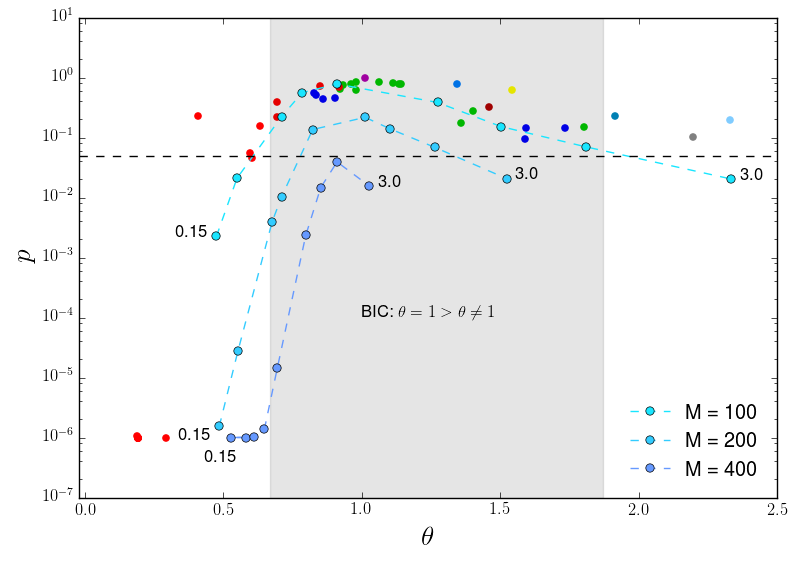
\includegraphics[width=0.95\textwidth]{figs_io/theta_pval_model_orig.png}
  \caption{Comparison of the Random Economies with real data in the
    $(p, \theta)$ plane. The model is shown for three quantity of goods
    $M$, each curve represents the model results with the number of firms per good $n = N/M$ varying from 0.15 to 3. We observe that the model parameters are able to represent the range of economies well, however these results are not scale dependent, not converging to a well defined limit when we increase $M$ keeping $n$ constant.}
  \label{fig:theta_pval_model_orig}
\end{figure}


The Use and Make tables can be defined for the Random Economies as
a function of the price vector $p$, the scales of production $s$ and the technologies $\xi$. The total amount of a good $\mu$ a firm $i$ produces is given by $p_\mu s_i \xi_i^\mu$ for all goods $\mu$ that have positive $\xi_i^\mu$. Likewise, the amount used is given by the negative terms in $\xi_i$. We define them the Use and Make tables as:

\begin{equation}
  \label{eq:io_4}
  U_{i\mu} = p_\mu s_i \left|\xi_i^{\mu, -}\right|, \quad M_{i\mu} =
  p_\mu s_i \xi_i^{\mu, +},
\end{equation}
where $\xi_i^{\mu,+} = \xi_i^\mu$ if $\xi_i^\mu > 0$ and $0$
otherwise. Likewise, $\xi_i^{\mu, -} = \xi_i^\mu$ only if
$\xi_i^\mu < 0$. One thing to note is that, unlike real Input-Output data, in
the model a good is never used as an input to itself. Therefore either $M_{i\mu}$ is positive or $U_{i\mu}$, never
both and $D_{\mu\mu} = 0$ for all goods, unlike the data where the
diagonal terms of the $D$ are usually large. Yet this holds only at the
microscopic level: for the model, $D_{\mu,\mu}$ can be nonzero after
aggregation.


We observe in numerical simulations that the properties of the model's direct requirement matrices are similar to the
real world data. For $M=100$, the degree distributions of the random
economies are remarkably similar to the ones given by real data, if we
vary $N$ (and therefore $n$), as shown in Figure
\ref{fig:theta_pval_model_orig}. When the repertoire of technologies is
relatively small (small $N$) compared to the number of goods, the
model exhibits a broad distribution of degrees reminiscent of the US
data whereas when $N$ increases the distribution becomes less heavy
tailed. However, as can be seen in Figure \ref{fig:theta_pval_model_orig}, these degree distributions are dependent on the
parameters $M$, $N$ and $\epsilon$ in a complicated manner and do
not converge to a well defined limit as $M$ diverges with $n=N/M$ and
$\epsilon$ finite.

Yet the behavior of the model under aggregation is quite similar to
that observed in real data, as seen in Figure
\ref{fig:theta_pval_model_agg} and degree distribution converges to
the same cluster of noninformative exponential distributions of the EU
/ US aggregated data.

\begin{figure}[!ht]
  \centering
  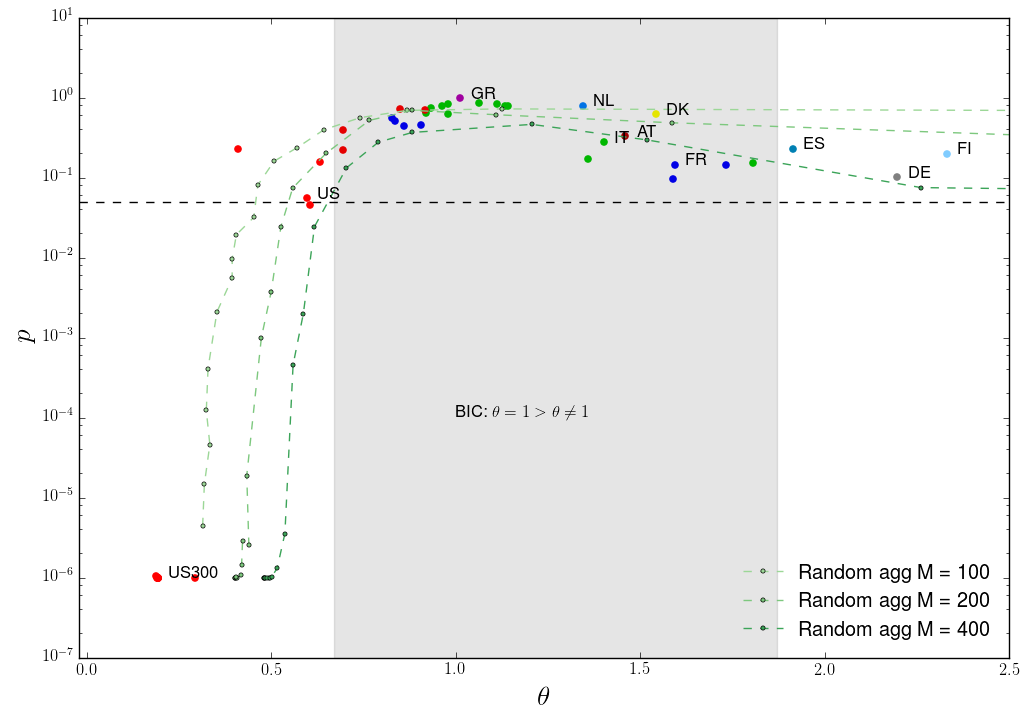
\includegraphics[width=0.95\textwidth]{figs_io/theta_pval_model_agg.png}
  \caption{Comparison of the randomly aggregated Random Economies with real data in the
    $(p, \theta)$ plane. The model always starts at one single
    realization of the Make and Use tables (as opposed to averaged
    over the disorder) for $n=0.15$ and randomly aggregated.}
  \label{fig:theta_pval_model_agg}
\end{figure}


\subsection{Consequences of aggregation}

The above results provide good evidence that the method by which the
BEA aggregates the sectors in the US economy is closer to a random
aggregation that to a ranked one. The Eurostat has no data publicly
available for a higher level of disaggregation, yet comparing the
degree distributions at the $M\sim 64$ sectors level suggests that EU
aggregation is also performed in an effectively random manner. In this
section we explore the consequences of this washing out of
information.

The direct requirement graph allows us to characterize the structural
susceptibility of the economy to shocks and perturbations: the
distribution of degrees give us a notion of how asymetric are the
dependencies between goods and what fraction of the production
capabilities depend on a single (or a few) goods. One of the ways
aggregation can lose information is if it doesn't take the good
degrees into account when selecting pairs to merge. Then, it will
likely happen that high degree goods will be aggregated with low
degree goods, possibly creating a good that has an degree in between the original ones\footnote{One must keep in mind that because aggregation is linear on the Use and Make tables, not in the Direct Requirement table, it's not true that the good resulting from the aggregation of a set of goods will have degree equal to the average of this set.}. This will gradually be responsible for eliminating the heavy tail of the distribution, masking the very high dependencies which are the most important for determining shock volatility. We test this hypothesis by calculating the normalized standard deviation of the ranks bundled together at each step: we define the rank of a good as its position in an ordered list of degrees, 1 being the lowest degree good and $M$ the highest degree good, then given a new good $\mu' = \sum_{k=1}^K \mu_k$ and given by  $r(\mu)$, then we the standard deviation of the aggregation as

\begin{equation}
    \frac{\sigma(\mu')}{M} = \frac{1}{M} \sqrt{\sum_{k=1}^M \left(r(\mu_k) - \bar{r}\right)^2}
\end{equation}

The results of $\frac{\sigma}{M}$ for each bundle of goods aggregated at each step using the three methods are shown in Figure \ref{fig:chi}. One sees that, as expected, this spread in the degrees being aggregated is highest when the random method is used and lowest when rank based is used, with the actual category based classification in between.

The degrees, however, are a first order measure for the spread of
perturbations which does not take cascade effects into account: the
perturbation of a good will impact the production of its dependencies
which may also have very high degree, amplifying the initial shock. In
\cite{Acemoglu12}, the authors show that the norm of a quantity similar to
the Bonacich centrality vector \cite{JacksonBook} is a lower bound for
the aggregated fluctuations generated by random, independent shocks
acting on the whole economy. This vector is given by

\begin{equation}
  \label{eq:centrality}
  \chi = \frac{\alpha}{M}(\mathds{I} - (1-\alpha) D)^{-1}\cdot \mathds{1},
\end{equation}
where $\mathds{I}$ is the identity matrix, $\mathds{1}$ is a vector
with all entries equal to one and $\alpha \in (0,1)$. The argument
used by Acemoglu \emph{et al} in \cite{Acemoglu12} is that in a
balanced structure in which random independent shocks in the whole
network average themselves out, as $M$ increases the norm
$\|\chi\| (M)$ of the vector should decrease proportionally to $\sqrt{M}$, but if
one calculates the $\chi$ both for the $M=382$ and $M=71$ aggregation
levels of the BEA data, the decrease is approximately
$~n^{\frac{1}{8}}$, considerably slower than a balanced economy. This
is interpreted as an evidence that the US economy is more susceptible
than expected to shocks.

\begin{figure}[!ht]
  \centering
  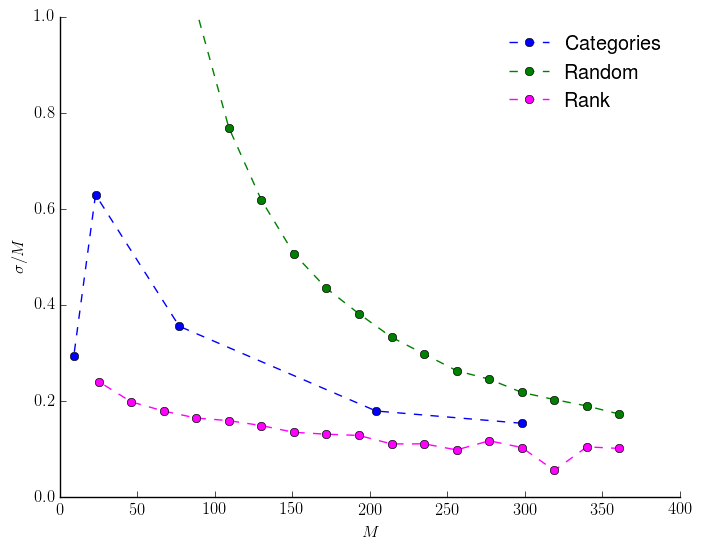
\includegraphics[width=.48\textwidth]{figs_io/cv_degree.png}
  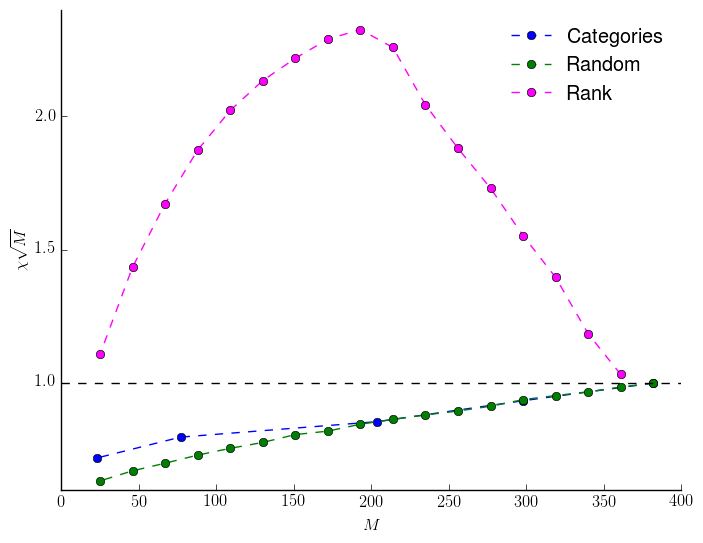
\includegraphics[width=.48\textwidth]{figs_io/susc_data.png}
  
  \caption{\textbf{(Left)} Scaled standard deviation $\sigma / M$ for
    the degree rank of the goods that are considered a single good at
    each aggregation step. The random aggregation has the highest
    average standard deviation, while the rank based has the
    lowest. This further corroborates the idea that random (and
    category) aggregation washes out high dependencies by merging them
    with low ones. \textbf{(Right)} Normalized average Bonacich
    centrality $\chi\sqrt{M}$ \cite{Acemoglu12}. This quantity should
    be constant if aggregated shocks have a limited effect (because
    $\chi$ decreases with $\sqrt{M}$) Here we see that networks with
    random aggregation have a different susceptibility to shocks than
    rank based ones, in particular, random (and category based)
    aggregation has $\chi$ decreasing slower than $\sqrt{M}$,
    exacerbating the effects of shocks.}
  \label{fig:chi}
\end{figure}


We calculate the same quantity for the three aggregation types
and plot the normalized (by $M=382$) $\|\chi\|\sqrt{M}$ on figure
\ref{fig:chi}. This quantity should be constant if $\|\chi\|$ decreases
proportionally to $\sqrt{M}$, as expected in a balanced structure, and
increasing with $M$ if it falls slower than that. We see on the graph
that random aggregation, again, generates a slightly unbalanced
structure, but the behaviour under rank aggregation is very different,
first increasing rapidly with $M$ (i.e., what would indicate a very
susceptible structure), but then it falls equally fast. We interpret
this result as a clear evidence that the direct requirement graph
properties are not simply a characteristic of the economy itself, but
very dependent on the method used for aggregation.

The important takeaway from this analysis is that sector
classification changes the whole structure of Direct Requirement
matrices. If the current classification methods serve a specific
purpose not related to the input-output structure, then when analysing
the Input-Output tables one must take into account that systemic risks like the
ones discussed in \cite{Acemoglu12} are aggregated away and
underrepresented.

However, if the purpose of building the Input-Output tables is to
make an assessment of which sectors are structural and which ones are
not, then the way the classification
hierarchy is built must change. The current one is, for a lack of better word,
``thematic''. Food is always aggregated together, so are the byproducts of
mining and so are services. These do not take into account the fact
that strawberries and eggs may have wildly different centralities and
degrees in the input-output network. The Spearman rank method we used
is a highly artificial way to aggregate, but it still preserves the
high degree of dependence of the US economy in certain crucial sectors.


\section{Conclusion}

The economic woes of the last decade brought to surface the importance
of identifying firms, and sectors, that are highly structural and from
which a sizeable portion of the production depends, and properly taking
steps to make the economy less vulnerable. However, we have shown here
that if one is not careful when organizing and classifying economic
data, this information can be lost.

Our results also show that at an intermediate scale of aggregation,
economies exhibit universal statistical properties that suggest that a
Statistical Mechanics approach may be feasible. In particular, the
study of the aggregation properties of models of large economies can
provide valuable hints on building a theory of macroeconomic
behaviour based on microeconomic interactions.

Going back to the question of what is the purpose of the current
classification scheme. From the BEA handbook we read

\begin{quote}
  The I-O tables are used to study changes in the structure of the
  U.S. economy and to assess the impact of specified events on
  economic activity.
\end{quote}

However, both the North American Industry Classification System
(NAICS), used by the BEA to construct the US data, and the NACE, used
by Eurostat, have as main purpose and advantage the usage of a uniform
classification for all the countries and their respective statistical
agencies in North America and the European Union. It is not surprising,
therefore, that the effects of their aggregation are closer to a
random process than to a method that takes the underlying data structure into
account.
